\section{结果}

\subsection{大NA、高透过率、宽带工作的二阶微分超表面}

本文重点讨论这一二阶傅里叶微分任务，是因为它同时要求大NA、高透过率、宽带工作，并且还要兼顾响应曲率、中心抑制、外角度幅值保持以及图像域算子行为。二阶验证分数是在 $T_{pp}$ 角谱行上逐波长计算的。结果非常典型：全数据集的平均分数只有约 $0.15$--$0.17$，但顶级候选在 1050 和 1100~nm 可以超过 $0.93$。这说明可行解集并不密集，呈现出“稀疏但真实存在”的特征，因此更适合用生成式候选探索来处理。

在 1050 和 1100~nm 处，最优二阶结果的验证分数都超过了 $0.93$；1150~nm 附近也出现了一组超过 $0.925$ 的高质量结果。之所以强调这些代表性结果，是因为它们同时展现出接近理想二阶响应的中心低谷、对称外扬角谱，以及较高角度下仍然可用的传输幅值。

\begin{figure}[!htbp]
\centering
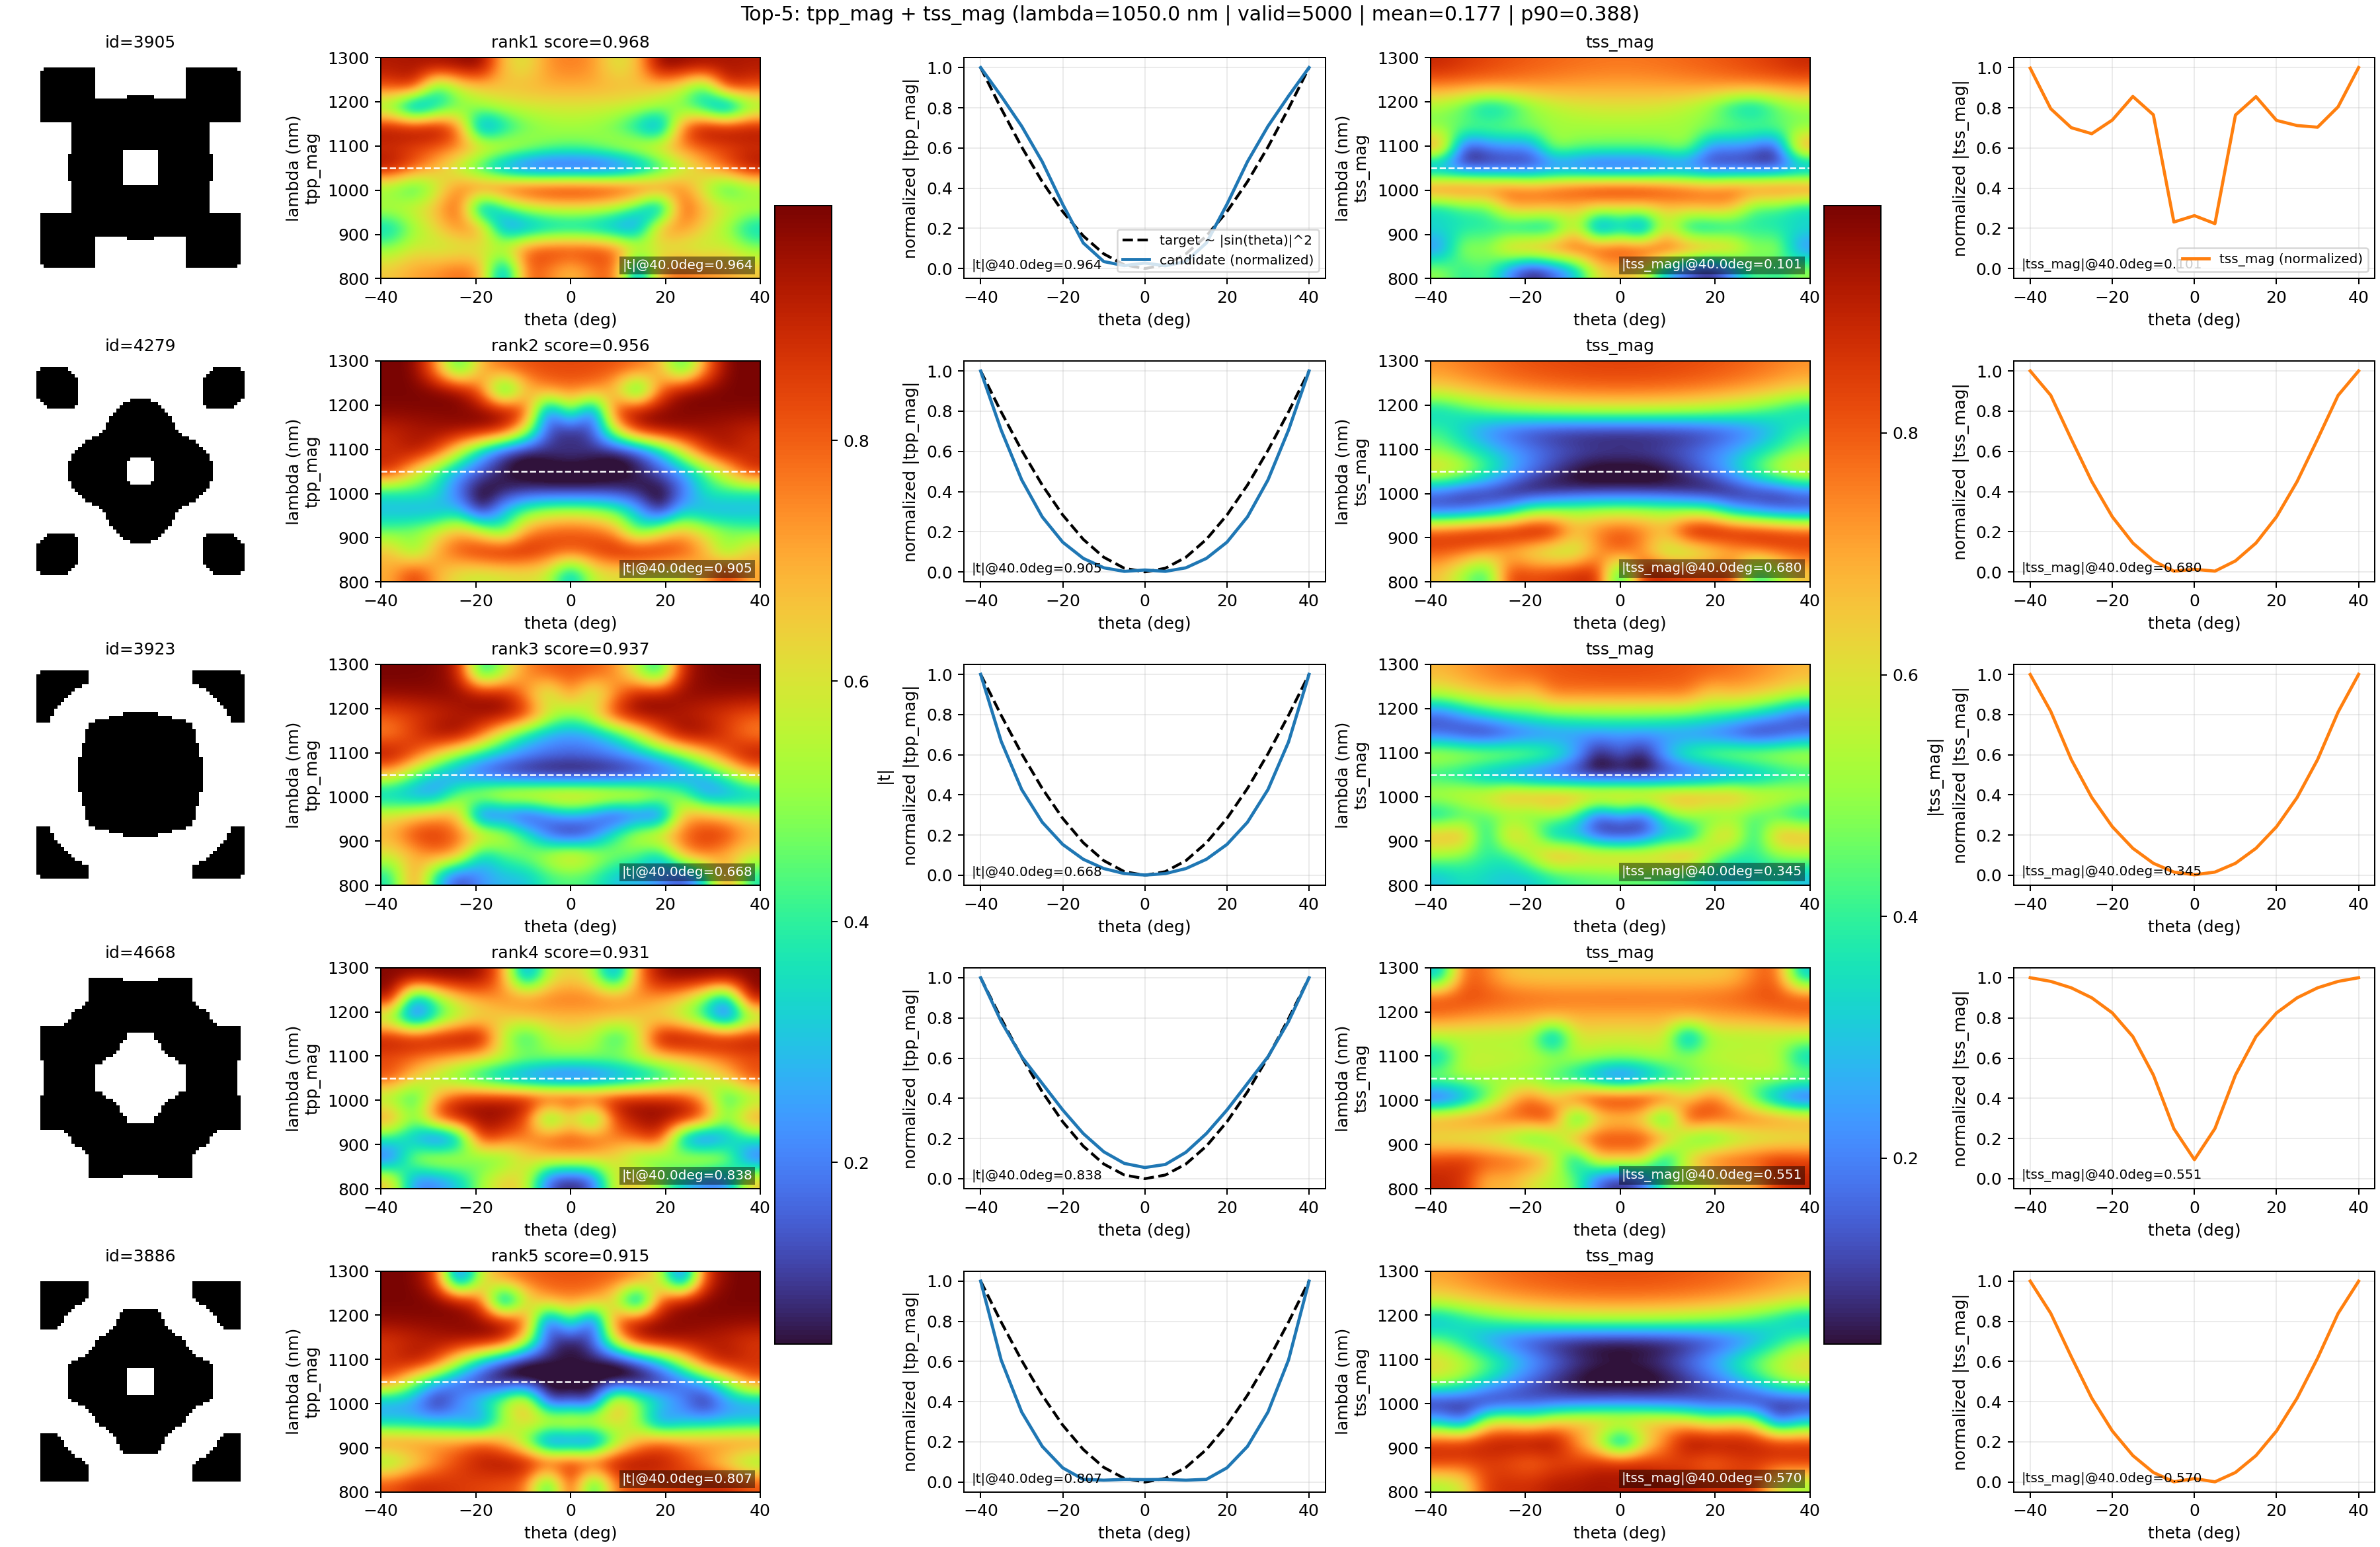
\includegraphics[width=0.78\linewidth]{../data/second_order_scores/tpp_mag_top5_plots/lambda_1050.0nm_top5.png}
\caption{1050~nm 处二阶微分任务的 top-5 排名图。这个结果展示了高质量算子响应在数据集中的集中分布。}
\label{fig:second1050}
\end{figure}

图~\ref{fig:second1050} 给出了 1050~nm 时的 top-5 候选，其中排名最前的结果已经呈现出代表性的二阶响应。它的重要性不只是“分高”，更在于它的验证响应在有限角度窗口内保持了明显的二阶算子几何，因此具有真实的算子解释力。相近的高质量响应在独立评估中反复出现，也说明这些高分结果对应的是验证响应流形上最稳定的强解区域。

在文献对比层面，二阶结果也是本文最适合展开性能定位的部分。按照本文统一采用的下游成像分析口径，1050~nm 的最优结果对应的综合分数约为 $0.988$，边缘幅值比约为 $0.97$，有效工作带宽约为 $100$~nm，数值孔径约为 $0.64$。这使它可以和近期强调 broadband、高 NA、高效率的微分超表面工作进入同一讨论语境 \cite{cotrufo2023natcom,deng2024,qiu2025highorder,zhou2025laplace}。本文在这里更想强调的是，同一 response-centered 设计框架既能得到这种高性能二阶行为，也能自然推广到偏振和时空目标。

\begin{figure}[!htbp]
\centering
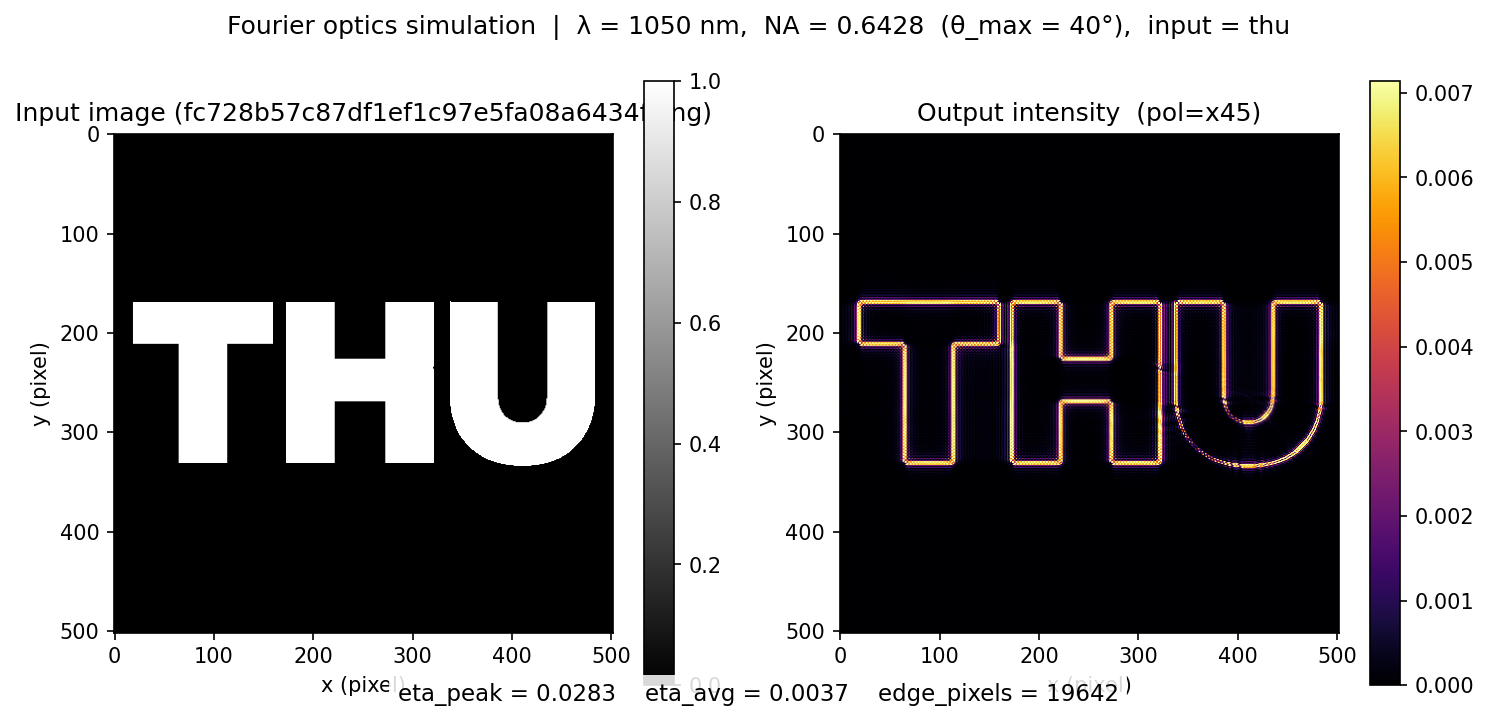
\includegraphics[width=0.63\linewidth]{../src/infer/results/p/1050nm_id4279/run_imaging_p_1050nm_id4279_1050nm_from_kspace_x45_thu_20260405_162600/imaging_result.png}
\caption{1050~nm 领先二阶结果的图像域验证。响应级的拟合已经转化成了清晰的边缘增强行为，而不只是停留在数值分数上。}
\label{fig:imaging}
\end{figure}

图~\ref{fig:imaging} 进一步把讨论从响应空间推进到了图像空间。当把验证得到的传递函数重新放回成像链路时，输出确实表现出典型的二阶微分效应：低频背景被压制，边缘和曲率敏感特征被突出。这一步非常关键，因为它说明本文方法恢复的是具有可解释光学作用的算子超表面，不是仅仅对分数函数拟合得很好的某类结构。

\begin{table}[!htbp]
\centering
\caption{本文正文反复使用的代表性验证结果。表中分数对应的是任务相关的验证排序，而非抽象的模型置信度。}
\label{tab:cases}
\begin{tabular}{>{\raggedright\arraybackslash}p{3.3cm}c>{\raggedleft\arraybackslash}p{2.2cm}>{\raggedleft\arraybackslash}p{4.1cm}}
\toprule
任务 & $\lambda$ (nm) & 主分数 & 说明 \\
\midrule
二阶微分 & 1050 & 0.9306 & 代表性 $T_{pp}$ 响应，兼具大NA与高透过率 \\
二阶微分 & 1100 & 0.9308 & 最强 1100~nm 验证结果 \\
偏振无关 & 1000 & 0.9358 & 双通道同时保持算子响应 \\
偏振复用 & 1100 & 0.7283 & active score $0.9348$，被动通道受抑 \\
四阶微分 & 1150 & 0.8884 & 外角度增长更陡 \\
低通 & 1050 & 0.9934 & 当前最强低通结果 \\
时空窗口 & 950 & 0.7271 & 验证筛选中的 merged 最优结果 \\
\bottomrule
\end{tabular}
\end{table}

\FloatBarrier

\subsection{向其他 OTF 目标的泛化}

在这一二阶结果之外，更重要的问题是：当目标响应形状发生变化时，这条 response-centered 闭环是否还能保持一致性。验证结果从三个维度给出了肯定答案。

第一维是偏振。偏振无关任务中，1000~nm 的最优结果联合验证分数达到 $0.9358$，1050 和 1100~nm 的领先结果也仍然保持在高分区间。这里的联合分数并非简单平均两个通道，它同时考虑各自的算子分数和 $\pm40^{\circ}$ 处的匹配程度。因此，同一框架能同时维持 $T_{pp}$ 与 $T_{ss}$ 的目标响应，说明偏振确实可以自然地作为一等设计维度进入条件张量。

第二维是偏振复用。当前最强的验证结果出现在 1100~nm，其 joint score 为 $0.7283$，但更关键的是 active-channel score 高达 $0.9348$，silent score 仍然保持在 $0.5218$。也就是说，这套方法不仅能保住一个通道的算子形状，还能显式暴露并优化“另一个通道需要尽量安静”这一目标。这正是统一响应张量应当揭示的通道级权衡。

\begin{figure}[!htbp]
\centering
\begin{minipage}[t]{0.48\linewidth}
\centering
\includegraphics[width=\linewidth]{../data/polarization_independent_scores/joint_top1_plots/lambda_1000.0nm_top1.png}
\end{minipage}\hfill
\begin{minipage}[t]{0.48\linewidth}
\centering
\includegraphics[width=\linewidth]{../data/polarization_multiplexed_scores/p_active_s_silent/p_active_s_silent_top5_plots/p_active_s_silent_lambda_1100.0nm_top5.png}
\end{minipage}
\caption{偏振相关泛化结果。左：1000~nm 的偏振无关最优 case。右：1100~nm 的偏振复用 top 候选。相同的逆向设计闭环既可以让两个通道对齐，也可以有意把两个通道分离。}
\label{fig:pol}
\end{figure}

第三维是目标形状的多样性。在四阶微分任务中，1050~nm 的最优分数达到 $0.9222$，而 1150~nm 的最强验证结果达到 $0.8884$。这说明当目标曲率比二阶更陡时，框架并没有失效。在低通任务中，1050~nm 与 1100~nm 的最优结果分别达到 $0.9934$ 和 $0.9863$，说明同样的 tensor conditioning 策略不仅能表达“多项式型角谱”，也能表达完全不同的通带型响应包络。

时空微分任务则是更强的压力测试，因为它直接在二维 wavelength--theta 窗口上评分，不再局限于单波长的一行曲线。当前 950~nm 的 dataset-level screen 给出了最高 merged score $0.7271$。考虑到它需要同时约束中心零线和窗口角落的角频联合结构，这个结果已经说明统一响应表述不仅是口头概念，也确实可以落入真实的验证评分过程。

\begin{figure}[!htbp]
\centering
\begin{minipage}[t]{0.48\linewidth}
\centering

\includegraphics[width=\linewidth]{../data/optica_lowpass_scores/tpp_mag_optica_lowpass_top5_plots/lambda_1050.0nm_top5.png}
\end{minipage}\hfill
\begin{minipage}[t]{0.48\linewidth}
\centering
\includegraphics[width=\linewidth]{../data/st2_template_match_20260330_233804/lambda_950nm/rank_001_sample_5409.png}
\end{minipage}
\caption{超出二阶微分之外的目标泛化。左：1050~nm 的低通 top 候选。右：950~nm 的时空窗口 top 候选。}
\label{fig:generalization}
\end{figure}

因此，图~\ref{fig:pol} 和图~\ref{fig:generalization} 支持的是同一个结论：本文的方法并非只对二阶微分有效，而是对应一条能够吸收通道要求、目标曲率、目标包络乃至目标支撑维度变化的统一 response-space 闭环。

\FloatBarrier

\subsection{模型对比与评估协议}

本文采用统一的 baseline 对比框架，覆盖 topology optimization、CVAE、cGAN 和 diffusion，并且全部在相同目标条件下、用同一套仿真后验证指标族比较。统一评测输出 best score、mean score、top-3 score、阈值成功率、spectrum MAE、binary rate、diversity 和 inference time。对当前问题来说，这种比较语言是合适的，因为强逆向设计器既要命中高质量样本，也要在可行集里生成足够多、足够多样且物理上有用的候选。

不过，就当前研究材料的保留情况而言，直接可用的 checkpoint 主要支持前向 surrogate 和 physics-guided diffusion 主线，而 cVAE、cGAN 与 topo-opt 并没有同步保留完整 checkpoint。表~\ref{tab:compare} 因此承担两个角色：一方面把正式对比协议写清，另一方面诚实记录当前直接可验证的模型证据，而不去编造缺失的 baseline 数字。

\begin{table}[!htbp]
\centering
\caption{本文使用的模型对比协议。所有核心指标都在仿真验证之后统计。只有直接保留下来的证据，才在表中填写具体数值。}
\label{tab:compare}
\begin{tabular}{>{\raggedright\arraybackslash}p{2.1cm}>{\raggedright\arraybackslash}p{2.4cm}>{\raggedleft\arraybackslash}p{2.1cm}>{\raggedleft\arraybackslash}p{2.1cm}}
\toprule
方法 & 条件 / 目标 & 直接保留证据 & 状态 \\
\midrule
Forward surrogate & structure $\rightarrow$ response，normalized $L_1$ & val loss $\approx 0.366$ & checkpoint + log 保留 \\
Diffusion & response $\rightarrow$ structure，扩散 + 物理 + 二值损失 & val loss $\approx 0.129$ & checkpoint + log 保留 \\
CVAE & response $\rightarrow$ structure，变分基线 & 统一评测接口已实现 & 本地缺 checkpoint \\
cGAN & response $\rightarrow$ structure，对抗式基线 & 统一评测接口已实现 & 本地缺 checkpoint \\
Topo-opt & task-guided iterative search & 统一评测接口已实现 & 旧依赖本地未补齐 \\
\bottomrule
\end{tabular}
\end{table}

即便如此，这一节仍然是有价值的。因为这一评估协议已经把“正确的比较问题”定义出来了：逆向模型必须在共享目标下比较验证 best-case score、平均候选质量、OTF MAE、二值程度和多样性。当前 physics-guided diffusion 主线是唯一带有可直接加载 checkpoint 的端到端保留方案，因此它自然成为本文的核心方法。
